\chapter{Plano de Trabalho - Projeto de Melhoria de Processos - Equipe SiGA}
\label{plano_de_projeto}
\section*{Escopo}

\subsection*{Objetivos}

\textbf{Necessidades do negócio:} 
Melhorar a qualidade dos produtos entregues.

\textbf{Motivações para melhoria:} 
\begin{itemize}
	\item Baixa qualidade dos produtos entregues;
	\item Dificuldades na implantação;
	\item Despadronização das formas de trabalho;
	\item Falta de monitoramento do projeto.
\end{itemize}

\textbf{Objetivos de melhoria:} 
\begin{itemize}
	\item Formalizar o processo de desenvolvimento de software;
	\item Otimizar a atividade de implantação;
	\item Estabelecer métricas para o processo.
\end{itemize}

\subsection*{Produtos Relevantes}

	Os produtos relevantes para o projeto de melhoria de processos da equipe SiGA são:
	
	\begin{itemize}
		\item Plano de Projeto de MPS;
		\item O processo de desenvolvimento de software;
		\item Cronograma;
		\item Estrutura analítica de risco;
		\item Relatório de Acompanhamento do projeto de MPS;
		\item Lista de melhorias.
	\end{itemize}


\section*{Recursos}

\subsection*{Recursos Humanos}

	Os recursos humanos alocados para o projeto são os dois desenvolvedores com dedicação total. Para orientação do projeto será alocado um orientador com disponibilidade para o projeto de 2 vezes por semana.


\subsection*{Recursos Materiais e de Infraestrutura}

	A equipe já possui os recursos materiais e de infraestrutura necessários para execução do projeto.

\section*{Cronograma}

\begin{figure}[!ht]
\centering
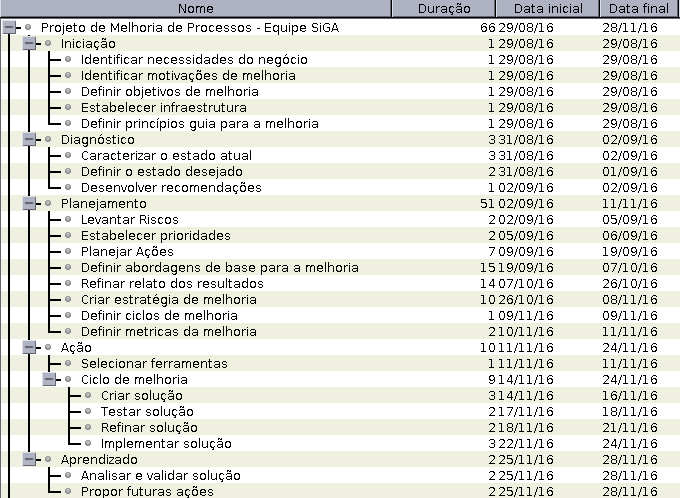
\includegraphics[scale=0.7]{figuras/cronograma.png}
\caption{Cronograma do projeto}
\label{fig:cronograma}
\end{figure}

\section*{Riscos}
  
  \subsection{Descrição dos processos de gerenciamento de riscos}

O Gerenciamento de Riscos possui processos definidos de seu planejamento, identificação, análise, planejamento de respostas e controle de riscos de um projeto \cite{pmbok}.
Para gerenciar os riscos do projeto, os processos adotados serão os seguintes:

\begin{itemize}
  \item \textbf{Identificar os riscos} - processos de identificação de riscos que podem afetar o desenvolvimento do projeto.
  \item \textbf{Realizar a análise qualitativa dos riscos} - processo de priorização dos riscos identificados para avaliação de sua probabilidade de ocorrência e análise de seu impacto.
  \item \textbf{Planejar as respostas aos riscos} - processo que determina respostas às ocorrências de riscos para diminuir seu impacto e para reduzir ameaças às fases de desenvolvimento do projeto.
  \item \textbf{Controlar os riscos} - processo que acompanha e monitora os riscos identificados, identifica novos riscos e avalia a eficácia do processo de gerenciamento de riscos em todas as fases de desenvolvimento do projeto.
\end{itemize}


\subsection{Qualificação dos riscos}
Os riscos identificados serão qualificados na sua probabilidade de ocorrência e impacto nos resultados, conforme as Tabelas \ref{probabilidade_riscos} e \ref{impacto_riscos} ilustram.

\begin{table}[h]
\centering
\caption{Probabilidade dos riscos}
\label{probabilidade_riscos}
\begin{tabular}{|l|l|}
\hline
\multicolumn{1}{|c|}{\textbf{Nível}} & \multicolumn{1}{c|}{\textbf{Descrição}} \\ \hline
Baixo                                & Muito improvável (0\% - 30\%)       \\ \hline
Médio                                & Pouco provável (31\% - 60\%)            \\ \hline
Alto                                 & Provável (61\% - 90\%)                  \\ \hline
\end{tabular}
\end{table}


\begin{table}[h]
\centering
\caption{Impacto dos riscos}
\label{impacto_riscos}
\begin{tabular}{|l|l|}
\hline
\multicolumn{1}{|c|}{\textbf{Nível}} & \multicolumn{1}{c|}{\textbf{Descrição}} \\ \hline
Baixo & Tem pouco prejuízo ao desenvolvimento do projeto \\ \hline
Médio & Prejudica o desenvolvimento do projeto, mas de rápida resiliência \\ \hline
Alto & Tem muito prejuízo ao desenvolvimento do projeto \\ \hline
\end{tabular}
\end{table}

\subsubsection{Prioridade dos riscos}

A prioridade dos riscos é dada pelo produto cartesiano da probabilidade e do impacto, conforme a Tabela \ref{prioridade_riscos}.

\begin{table}[h]
\centering
\caption{Classificação da Prioridade}
\label{prioridade_riscos}
\begin{tabular}{|
>{\columncolor[HTML]{9B9B9B}}c |
>{\columncolor[HTML]{34FF34}}c |c|
>{\columncolor[HTML]{FE0000}}c |}
\hline
\textbf{Provável} & \cellcolor[HTML]{FCFF2F}\textbf{Risco médio} & \cellcolor[HTML]{FE0000}\textbf{Risco alto} & \textbf{Risco extremo} \\ \hline
\textbf{Pouco provável} & \textbf{Risco baixo} & \cellcolor[HTML]{FCFF2F}\textbf{Risco médio} & \textbf{Risco alto} \\ \hline
\textbf{Muito improvável} & \textbf{Risco insignificante} & \cellcolor[HTML]{34FF34}\textbf{Risco baixo} & \cellcolor[HTML]{FCFF2F}\textbf{Risco médio} \\ \hline
\cellcolor[HTML]{656565}\textbf{Probabilidade/Impacto} & \cellcolor[HTML]{9B9B9B}\textbf{Baixo} & \cellcolor[HTML]{9B9B9B}\textbf{Médio} & \cellcolor[HTML]{9B9B9B}\textbf{Alto} \\ \hline
\end{tabular}
\end{table}

\subsubsection{Riscos Identificados}

Os riscos identificados para o projeto estão listados na Tabela \ref{riscos_projeto}.

\begin{table}[h]
\centering
\caption{Riscos Identificados para o Projeto}
\label{riscos_projeto}
\begin{tabular}{|l|l|l|c|}
\hline
\multicolumn{1}{|c|}{\textbf{Risco}}                                                                                                            & \multicolumn{1}{c|}{\textbf{Probabilidade}} & \multicolumn{1}{c|}{\textbf{Impacto}} & \textbf{Prioridade}                    \\ \hline
\begin{tabular}[c]{@{}l@{}}Não ser possível atender todos os \\ objetivos de melhoria propostos\end{tabular}                                    & Baixa                                       & Média                                 & \cellcolor[HTML]{34FF34}\textbf{Baixa} \\ \hline
\begin{tabular}[c]{@{}l@{}}Não conseguir a cooperação de toda \\ a equipe para o processo de melhoria\end{tabular}                              & Baixa                                       & Alto                                  & \cellcolor[HTML]{FCFF2F}\textbf{Média} \\ \hline
\begin{tabular}[c]{@{}l@{}}Não conseguir acesso a documentos ou\\ informações necessários para a definição\\  processo de melhoria\end{tabular} & Média                                       & Médio                                 & \cellcolor[HTML]{FCFF2F}\textbf{Média} \\ \hline
\begin{tabular}[c]{@{}l@{}}Um integrante da equipe de melhoria \\ abandonar o projeto\end{tabular}                                              & Baixa                                       & Média                                 & \cellcolor[HTML]{34FF34}\textbf{Baixa} \\ \hline
\begin{tabular}[c]{@{}l@{}}Projeto alvo de melhoria ser encerrado\\ por motivos maiores da organização\end{tabular}                             & Média                                       & Alto                                  & \cellcolor[HTML]{FE0000}\textbf{Alto}  \\ \hline
\end{tabular}
\end{table}

\subsubsection{Ações de resposta aos riscos}

As ações definidas para reagir aos riscos identificados se encontram na Tabela \ref{acoes_riscos}.

\begin{table}[h]
\centering
\caption{Ações de contingência aos riscos}
\label{acoes_riscos}
\begin{tabular}{|l|l|}
\hline
\multicolumn{1}{|c|}{\textbf{Risco}}                                                                                                            & \multicolumn{1}{c|}{\textbf{Ações de contingência}} \\ \hline
\begin{tabular}[c]{@{}l@{}}Não ser possível atender todos os \\ objetivos de melhoria propostos\end{tabular}                                    & Redefinir o escopo da melhoria                      \\ \hline
\begin{tabular}[c]{@{}l@{}}Não conseguir a cooperação de toda \\ a equipe para o processo de melhoria\end{tabular}                              & Motivar a equipe mostrando os benefícios da melhoria\\ \hline
\begin{tabular}[c]{@{}l@{}}Não conseguir acesso a documentos ou\\ informações necessários para a definição\\  processo de melhoria\end{tabular} & Levantar as informações necessárias por meio de diálogo \\ \hline
\begin{tabular}[c]{@{}l@{}}Um integrante da equipe de melhoria \\ abandonar o projeto\end{tabular}                                              & Redefinir o escopo para contemplar o tamanho da equipe \\ \hline
\begin{tabular}[c]{@{}l@{}}Projeto alvo de melhoria ser encerrado\\ por motivos maiores da organização\end{tabular}                             & Documentar o estado do processo de melhoria e entregá-lo \\ \hline
\end{tabular}
\end{table}

\section*{Plano de Comunicações Relevantes}

	\begin{itemize}
		\item Aprovação do processo definido;
		\item Acompanhamento do projeto;
		\item Divulgação dos resultados.

	\end{itemize}

\section*{Plano de Monitoramento}
	
	O monitoramento do projeto de MPS será realizado semanalmente juntamente com o orientador.

